\documentclass{protokol}
\usepackage{graphicx}
\usepackage{float}

\usepackage{tikz}
\usetikzlibrary{calc}
\usetikzlibrary{arrows}


%====== Units =====
\usepackage{amssymb}
\usepackage{siunitx}
\sisetup{inter-unit-product =\ensuremath{\cdot}}
\sisetup{group-digits = integer}
\sisetup{output-decimal-marker = {,}}
\sisetup{exponent-product = \ensuremath{\cdot}}
\sisetup{separate-uncertainty}
\sisetup{tight-spacing = false}
%\sisetup{scientific-notation = true}
%\sisetup{round-mode=places,round-precision=4}
%\sisetup{evaluate-expression}


%====== Grafy =====
\usepackage{pgfplots}
\pgfplotsset{width=0.8\linewidth, compat=1.17}
\def\plotcscale{0.8}
\usepackage{pgfplotstable}
\usepackage[figurename=Obr.]{caption} % figure caption rename

\usepackage[siunitx]{circuitikz} % obvody
% \ctikzset{bipoles/length=1cm}

%====== Rovnice align block ======
\usepackage{amsmath}
\setlength{\jot}{10pt} % rozestup mezi řádky

\graphicspath{ {./img/} }

%====== Code blocks ======
\usepackage{listings}

\usepackage[most]{tcolorbox}
\newtcbox{\inlinecode}{on line, boxsep=0pt, left=2pt, right=2pt, top=2pt, bottom=2pt, colframe=gray, boxrule=0.5pt, arc=1pt, auto outer arc, before upper={\vphantom{dlg}}, tcbox raise base} % vytvoření inline boxu pro kód

\lstdefinelanguage{Spice}{
    alsoletter={.},  % Přidává tečku jako součást slov
    morekeywords={.lib, .STEP, .param, .MEAS, FIND, WHEN, END, VALUE, R, C, L, K, .SUBCKT, .ENDS, .MODEL, .INCLUDE, .AC, .DC, .TRAN, .PRINT, .PLOT, .PROBE, .WIDTH, .OPTIONS, .NODESET, .IC},
    keywordstyle=\color{blue}\bfseries,
    sensitive=false, % klíčová slova nejsou citlivá na velikost písmen
    morecomment=[l]{;}, % komentáře začínají hvězdičkou
    morestring=[b]", % řetězce uzavřené do uvozovek
}

\lstset{
  language=Spice,
  basicstyle=\ttfamily\small,
  breaklines=true,
  numbers=left,
  numberstyle=\tiny\color{gray},
  frame=single,
  rulecolor=\color{black},
  title=\lstname,
  keywordstyle=\color{blue}\bfseries,
  commentstyle=\color{green},
  stringstyle=\color{red},
  showstringspaces=false
}

%====== Vyplňte údaje ======
\jmeno{Tomáš Vavrinec}
\kod{240893}
\rocnik{}
\obor{MET}
\skupina{}
\spolupracoval{--}

\merenodne{--}
\odevzdanodne{--}
\nazev{Způsoby lámání a spojování optických vláken}
\cislo{1} %měřené úlohy

\predmet{Optoelektronika a optické komunikace}
\ustav{Ústav mikroelektroniky}
\skola{FEKT VUT v~Brně}

\def\para{x+0}
\def\parb{\para-80}


%citace 
\usepackage[backend=biber, style=iso-numeric, sortlocale=cs_CZ, autolang=other, language=czech]{biblatex}
\addbibresource{bibliography.bib}
\DeclareFieldFormat{labelnumberwidth}{\mkbibbrackets{#1}}
% hyperlinky
\usepackage[colorlinks]{hyperref}

% odstavce
\usepackage{parskip}

% Bloky kódu
\usepackage{xcolor}

%New colors defined below
\definecolor{codegreen}{rgb}{0,0.6,0}
\definecolor{codegray}{rgb}{0.5,0.5,0.5}
\definecolor{codepurple}{rgb}{0.58,0,0.82}
\definecolor{backcolour}{rgb}{0.95,0.95,0.92}

\usepackage{listings}
\lstdefinestyle{mystyle}{
  backgroundcolor=\color{backcolour}, commentstyle=\color{codegreen},
  keywordstyle=\color{magenta},
  numberstyle=\tiny\color{codegray},
  stringstyle=\color{codepurple},
  basicstyle=\ttfamily\footnotesize,
  breakatwhitespace=false,         
  breaklines=true,                 
  captionpos=b,                    
  keepspaces=true,                 
  numbers=left,                    
  numbersep=5pt,                  
  showspaces=false,                
  showstringspaces=false,
  showtabs=false,                  
  tabsize=2
}
\lstset{
	inputencoding=utf8,
	extendedchars=true,
	literate={á}{{\'a}}1 {č}{{\v{c}}}1 {ď}{{\v{d}}}1 {é}{{\'e}}1 {ě}{{\v{e}}}1 
           {í}{{\'i}}1 {ň}{{\v{n}}}1 {ó}{{\'o}}1 {ř}{{\v{r}}}1 {š}{{\v{s}}}1 
           {ť}{{\v{t}}}1 {ú}{{\'u}}1 {ů}{{\r{u}}}1 {ý}{{\'y}}1 {ž}{{\v{z}}}1 
           {Á}{{\'A}}1 {Č}{{\v{C}}}1 {Ď}{{\v{D}}}1 {É}{{\'E}}1 {Ě}{{\v{E}}}1 
           {Í}{{\'I}}1 {Ň}{{\v{N}}}1 {Ó}{{\'O}}1 {Ř}{{\v{R}}}1 {Š}{{\v{S}}}1 
           {Ť}{{\v{T}}}1 {Ú}{{\'U}}1 {Ů}{{\r{U}}}1 {Ý}{{\'Y}}1 {Ž}{{\v{Z}}}1,
	style=mystyle
	}

% Číslování
\pagenumbering{arabic}



% =========================================
% =============== DOKUMENT ================
% =========================================
\begin{document}
	%====== Vygenerování tabulky ======
	\maketitle

\section*{ZADÁNÍ ÚLOHY}
  Detailní popis jednotlivých úloh s návodem najdete v NAO\_PC.pdf, který je dostupný v E-learningu.

\begin{itemize}
    \item {\bf Simulací získejte hodnoty prahového napětí \(U_{TH0}\) pro dvě různé řady rozměrů tranzistorů.}
    \begin{itemize}
        \item konstantní poměr \(W/L = 5, kdy \$L\$ = 0.18; 0.3; 0.5; 0.8; 1; 2; 3; 5; 10\),
        \item různé rozměry: \(W/L = 0.22/0.18; 1/0.5; 2/0.5; 2/1; 5/1; 5/2; 10/5; 10/10; 40/10\),
        \item výše uvedené dva body budou provedeny pro tranzistor NMOS i PMOS.
    \end{itemize}
    \item {\bf Závislost prahového napětí \(U_{TH}\) na \(U_{SB}/U_{BS}\) (bulk efekt) Simulací získejte hodnoty prahového napětí \(U_{TH}\) pro napětí \(U_{BS}\) (NMOS) resp. \(U_{SB}\) (PMOS) v rozsahu \(0 [V]\) až \(500 [mV]\) s krokem \(50 [mV]\).}
    \item {\bf Závislost parametru modulace délky kanálu (\(\lambda\)) na délce kanálu (L) Simulací získejte hodnoty parametru \(\lambda\) tranzistoru NMOS a PMOS pro L v rozmezí \(200 [nm]\) až \(10 [\mu m]\).}
\end{itemize}

\subsection*{Bonusové otázky (1 b.)}
\begin{itemize}
    \item Popište, jak byste simulací (mimo analýzu \inlinecode{.op}) zjistili transkonduktanci \(gm\).
          Nakreslete schéma, popište nastavení a odečet hodnot.
\end{itemize}

\setcounter{section}{0}

\newpage
\section{Lámání Vláken}
  Nejprve je nutné optické vlákno zbavit ochrany, jak sekundární tak primarni.
  To bylo provedeno pomocí přiložených kleští a následně bylo očištěno izopropyl alkoholem.
  
  \begin{figure}[h!]
    \centering
    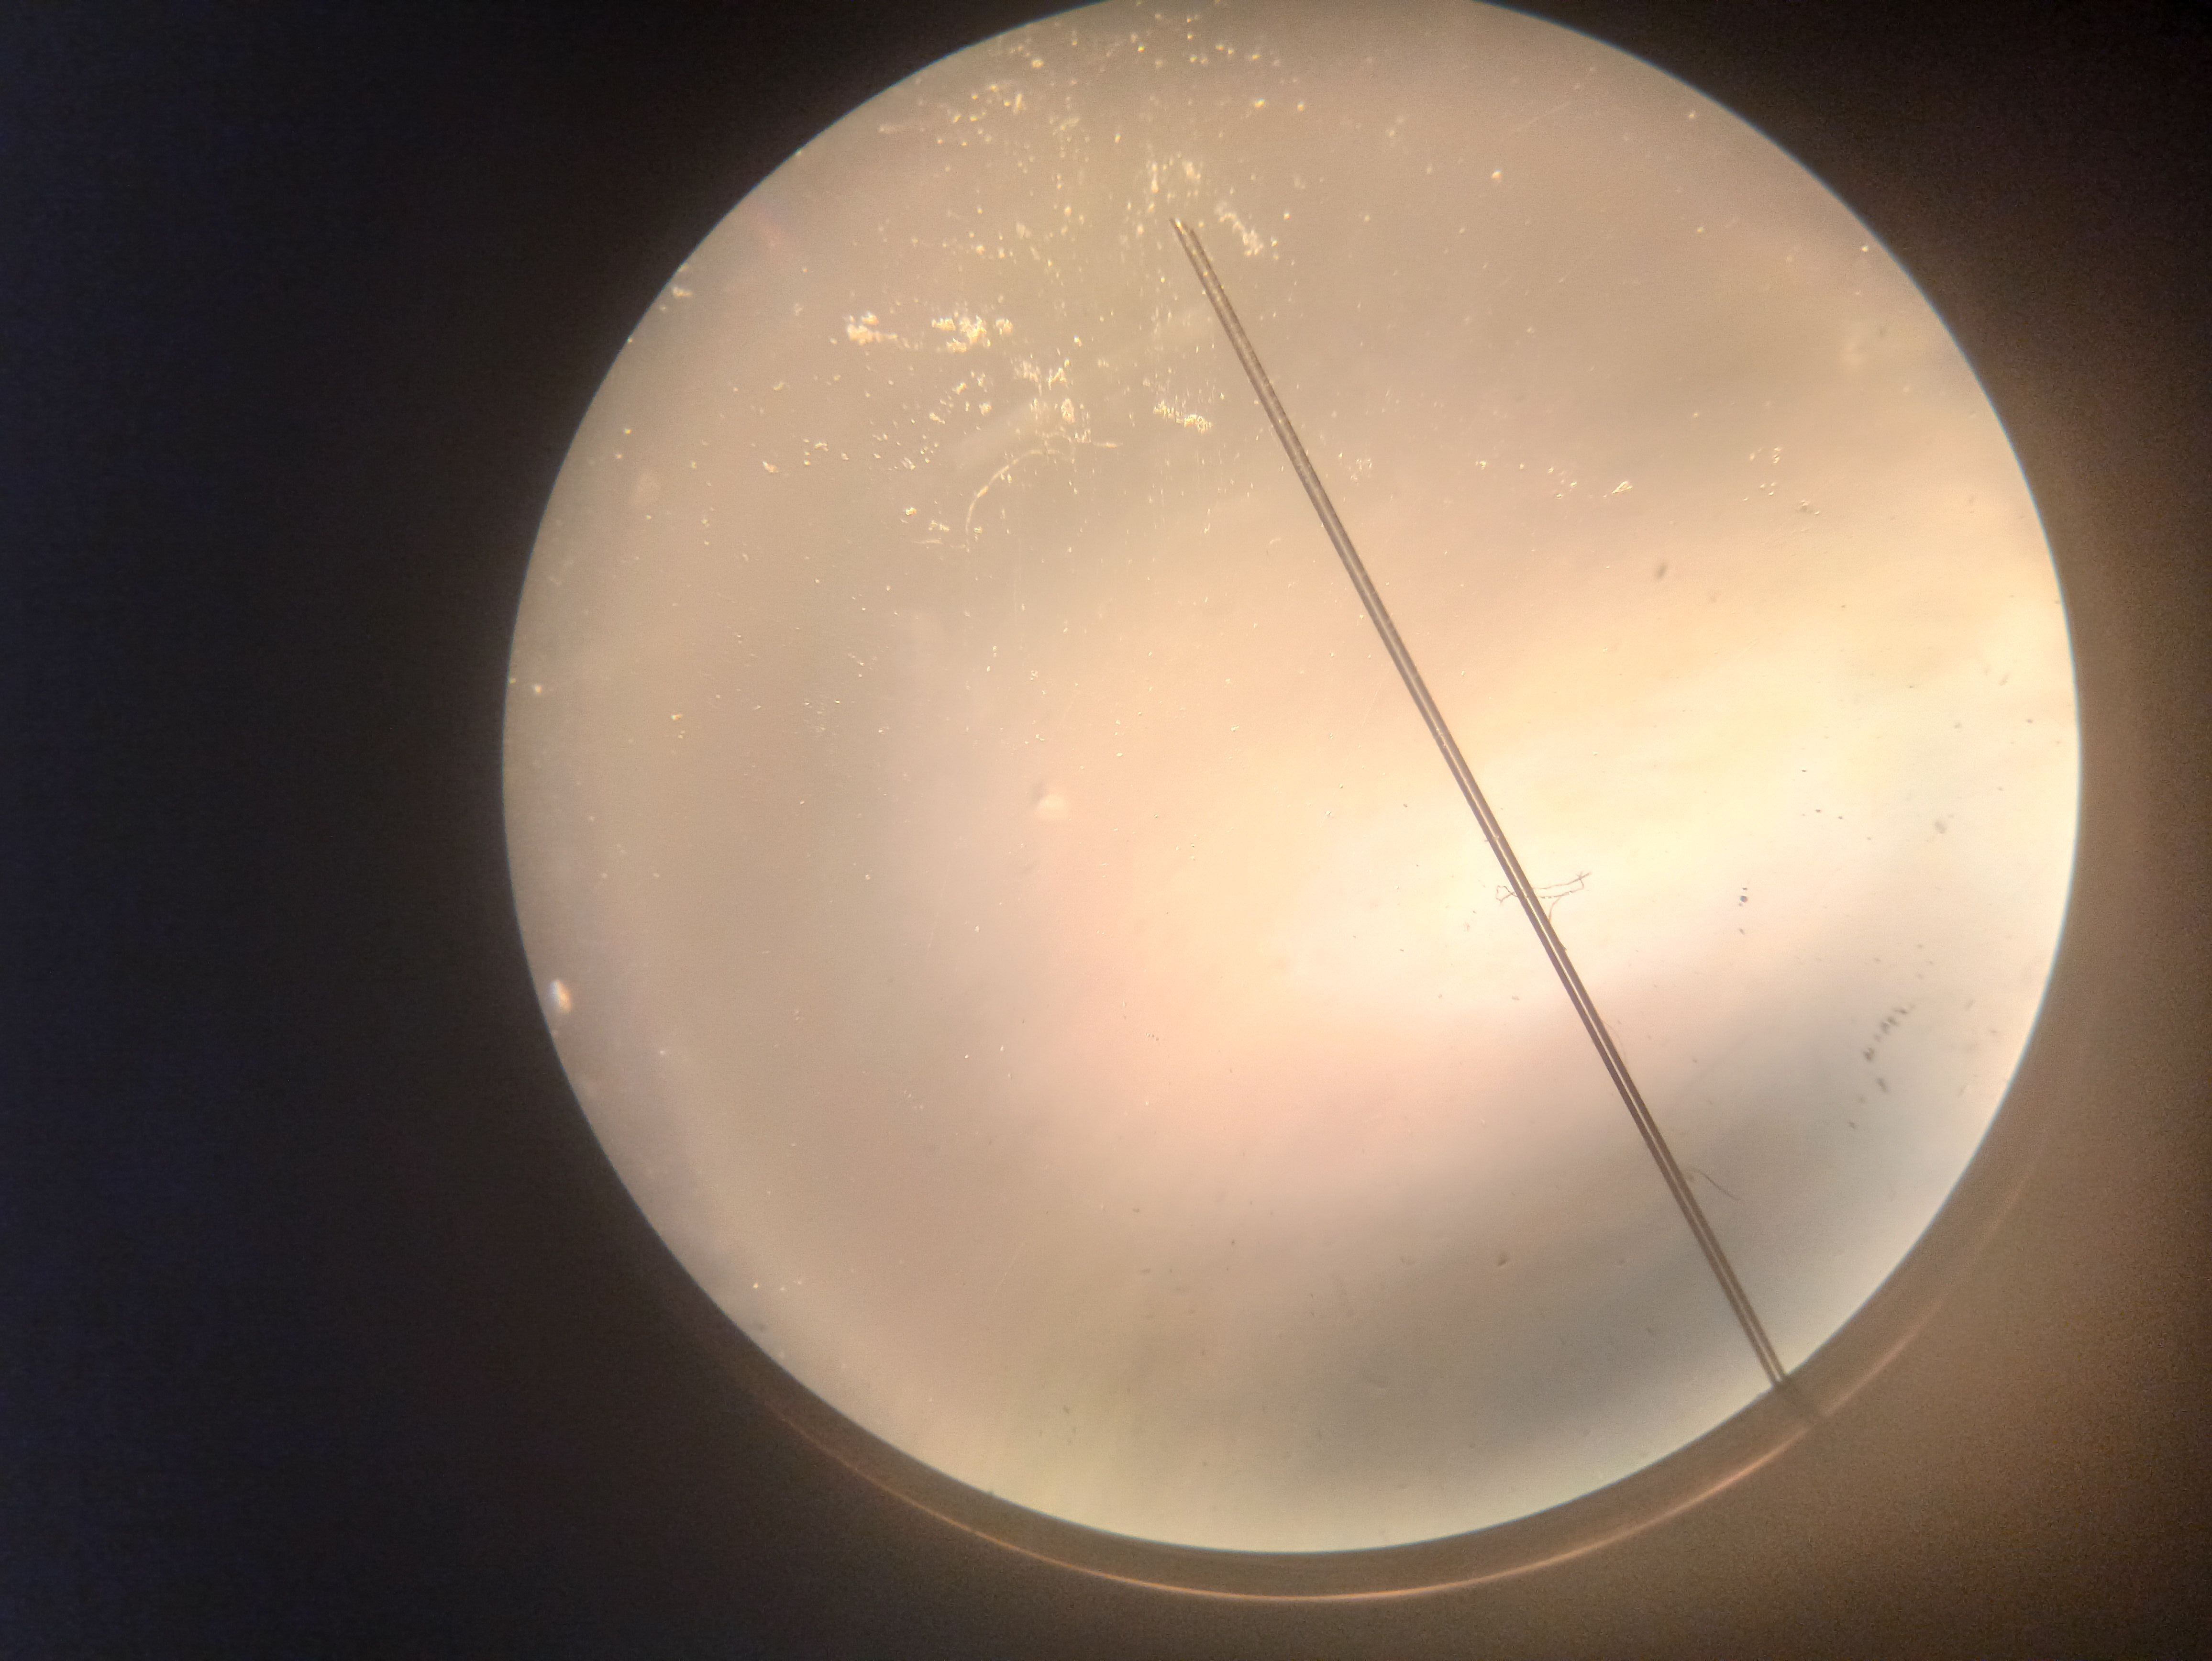
\includegraphics[width=0.6\textwidth]{text/img/odizolovano.jpg}
    \caption{\label{fig:odizolovano} Pohled mikroskopem na očištěné vlákno zbavené izolace}
  \end{figure}
  
  \subsection{Lamačka s diamantovým kotoučem}
    Vlákno zbavené ochrany bylo vloženo do lamačky a zlomeno.
    Následně bylo opět vloženo pod mikroskop, výsledek je viditelný na obrazcích \ref{diamKot} a \ref{diamKot_O}
    Jak je vidět výsledný lom nedosahuje dostatečné kvality pro optický spoj, ale ani po opakovaném pokusu se výsledek znatelně nezlepšil.  

    \begin{figure}[h!]
      \centering
      \includegraphics[width=0.6\textwidth]{text/img/diamantovyKotouc.jpg} 
      \caption{\label{fig:diamKot} Pohled mikroskopem na vlákno zlomené diamantovým kotoucem}
    \end{figure}

    \begin{figure}[h!]
      \centering
      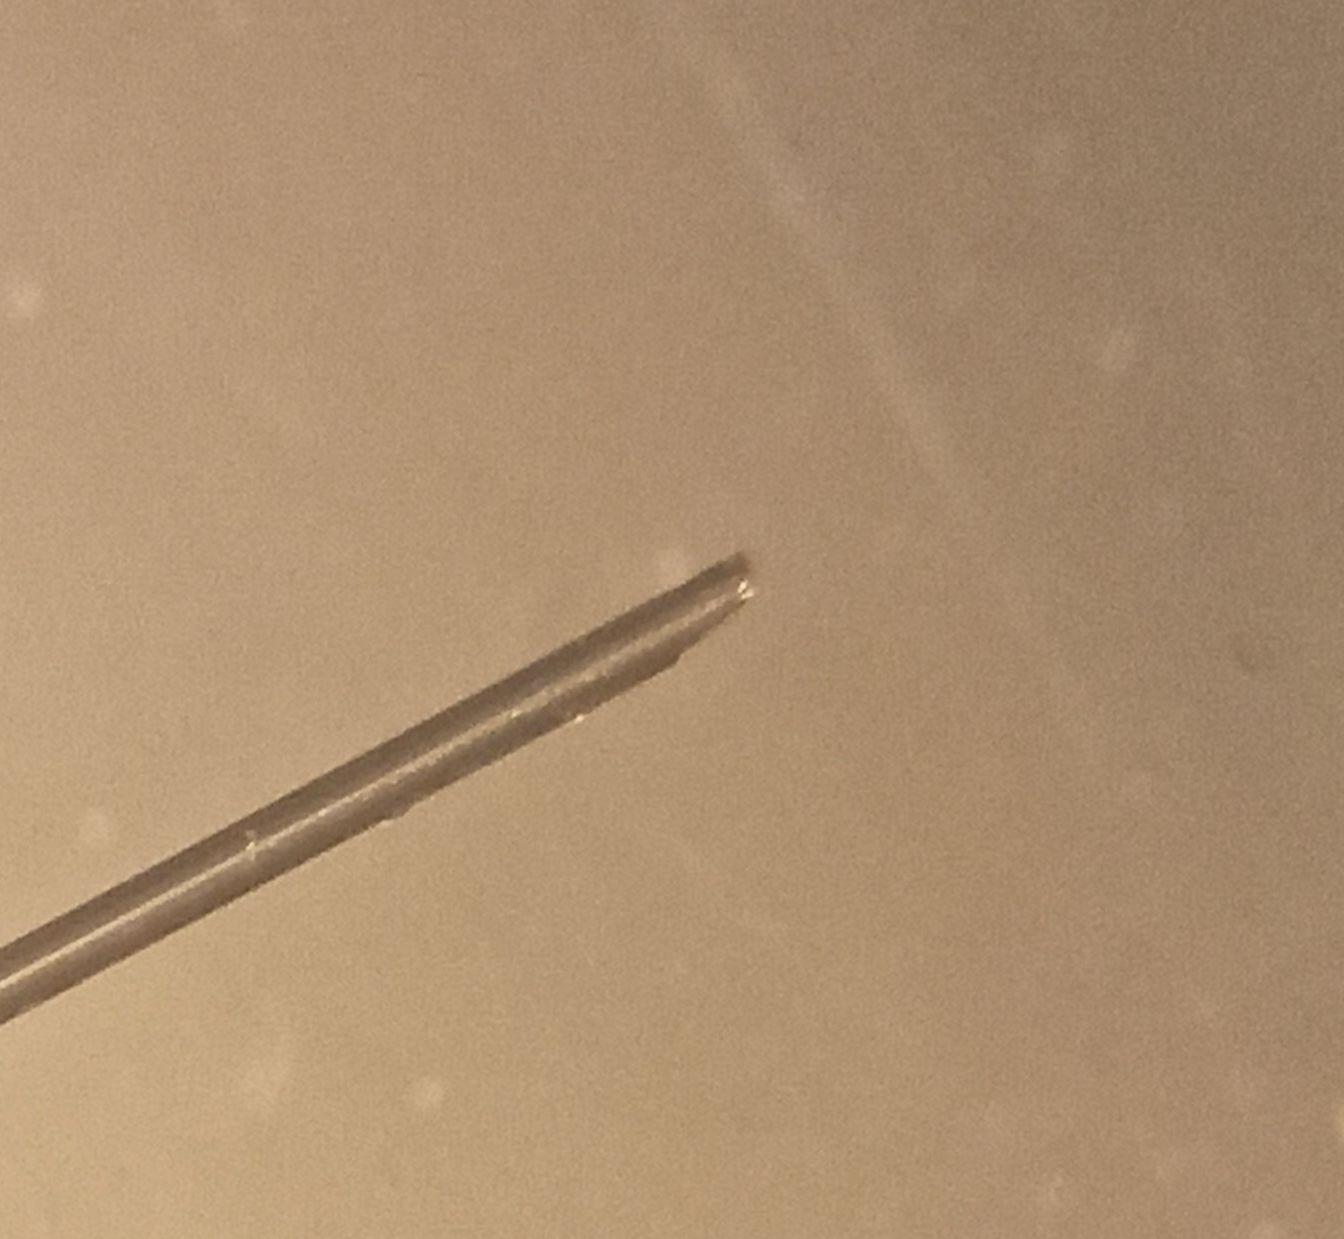
\includegraphics[width=0.6\textwidth]{text/img/diamantovyKotouc-O.jpg}
      \caption{\label{fig:diamKot_O} Oříznutý pohled na vlákno zlomené diamantovým kotoucem}
    \end{figure}

  \newpage
  \clearpage

  \subsection{Lamačka s diamantovým nožem}
    Obdobný postup byl aplikován u lamačky s diamantovým nožem.

    \begin{figure}[h!]
      \centering
      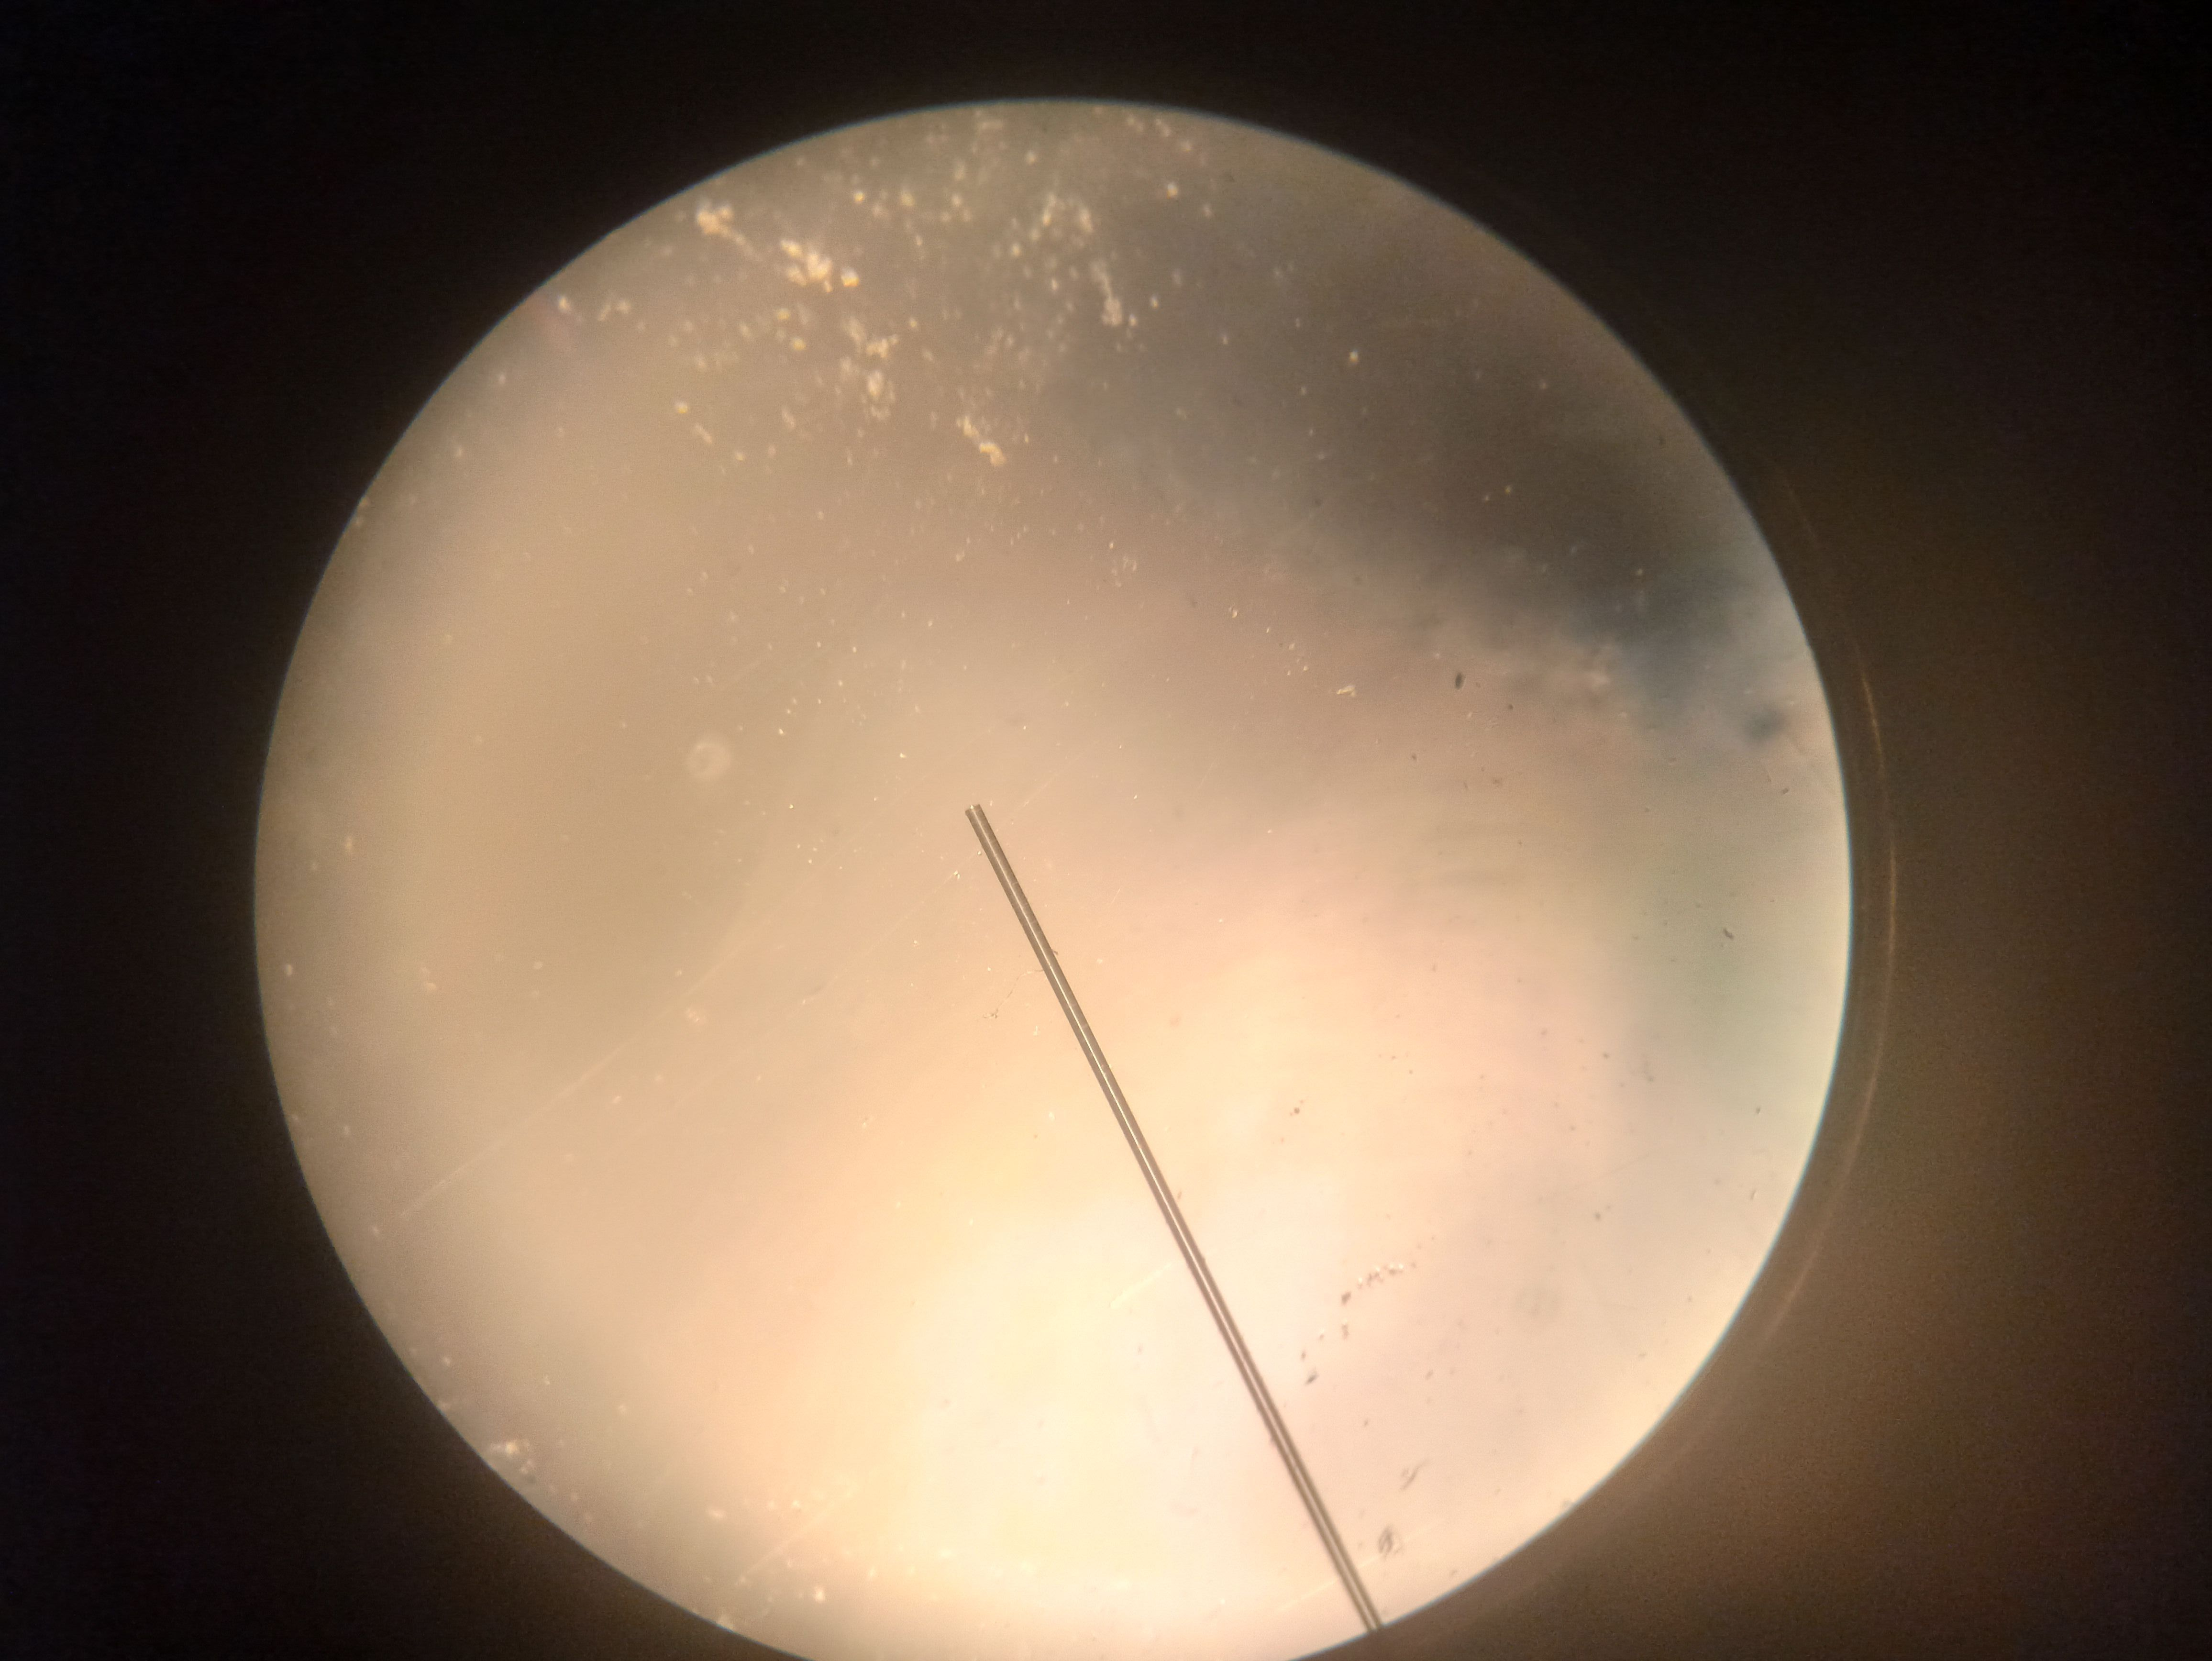
\includegraphics[width=0.6\textwidth]{text/img/diamantovyNuz.jpg} 
      \caption{\label{fig:diamNuz} Pohled mikroskopem na vlákno zlomené diamantovým nozem}
    \end{figure}

    \begin{figure}[h!]
      \centering
      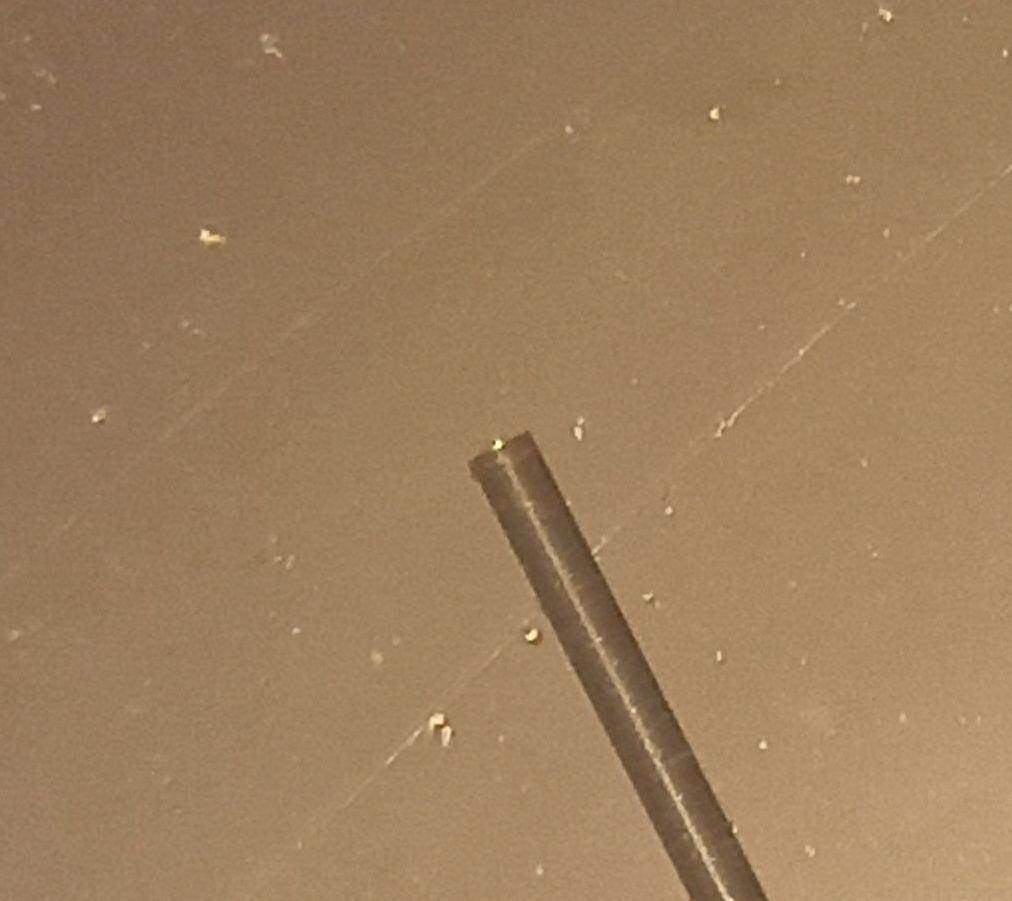
\includegraphics[width=0.6\textwidth]{text/img/diamantovyNuz-O.jpg}
      \caption{\label{fig:diamNuz-O} Oříznutý pohled na vlákno zlomené diamantovým nozem}
    \end{figure}

  \newpage
  \clearpage

  \subsection{Lom se safírovým nožem}

  \begin{figure}[h!]
    \centering
    \includegraphics[width=0.6\textwidth]{text/img/safirovyNuz.jpg} 
    \caption{\label{fig:safirNuz} Pohled mikroskopem na vlákno zlomené safírovým nozem}
  \end{figure}

  % \newpage
  % \clearpage

  \subsection{Lom se safírovou destičkou}

    \begin{figure}[h!]
      \centering
      \includegraphics[width=0.6\textwidth]{text/img/safirovaDesticka2.jpg} 
      \caption{\label{fig:safirNuz} Pohled mikroskopem na vlákno zlomené safírovou destičkou}
    \end{figure}

  

  \newpage
  \clearpage

  \section{Závěr}
    Porovnání obou verzí zesilovače.

\begin{table}[h]
    \centering
    \begin{tabular}{|l|c|c|c|}
        \hline
        \textbf{Typ zátěže} & \textbf{Zesílení \(A_{U0} [-]\)} & \textbf{Rychlost přeběhu  \(SR_{fell} [V/\mu s]\)} & \textbf{šířka pásma \(GBW [MHz]\)} \\ \hline
        Odporová            & 19                               & 3.5                                                & 8.43                               \\ \hline
        Aktivní             & 38                               & 5.0                                                & 8.12                               \\ \hline
    \end{tabular}
    \caption{Porovnání obou typů zátěže}
    \label{tab:zrcadla}
\end{table}

% \clearpage
% \section*{Reference}
% \printbibliography[heading=none]

\end{document}